% =============================================================
%  SECTION: Diagnostic and Stability Analysis
% =============================================================

\newpage
\section{Diagnostic and Stability Analysis}

Before extracting physical properties, we must verify that the simulation
is numerically stable and physically valid. A simulation can produce
perfectly self-consistent but entirely wrong results if the integrator
is poorly chosen or the timestep is too large. Three criteria must be
satisfied before we trust any output.

\subsection{Energy Conservation}

In the NVE ensemble (constant Number of atoms, Volume, and Energy), the
total energy $\Estar = K^* + U^*$ must be conserved. This is the most
sensitive test of the integrator's correctness. If $\Estar$ drifts
upward or downward monotonically, the timestep $dt^*$ is too large and
energy is being injected or extracted artificially by the integrator.

\begin{figure}[H]
    \centering
    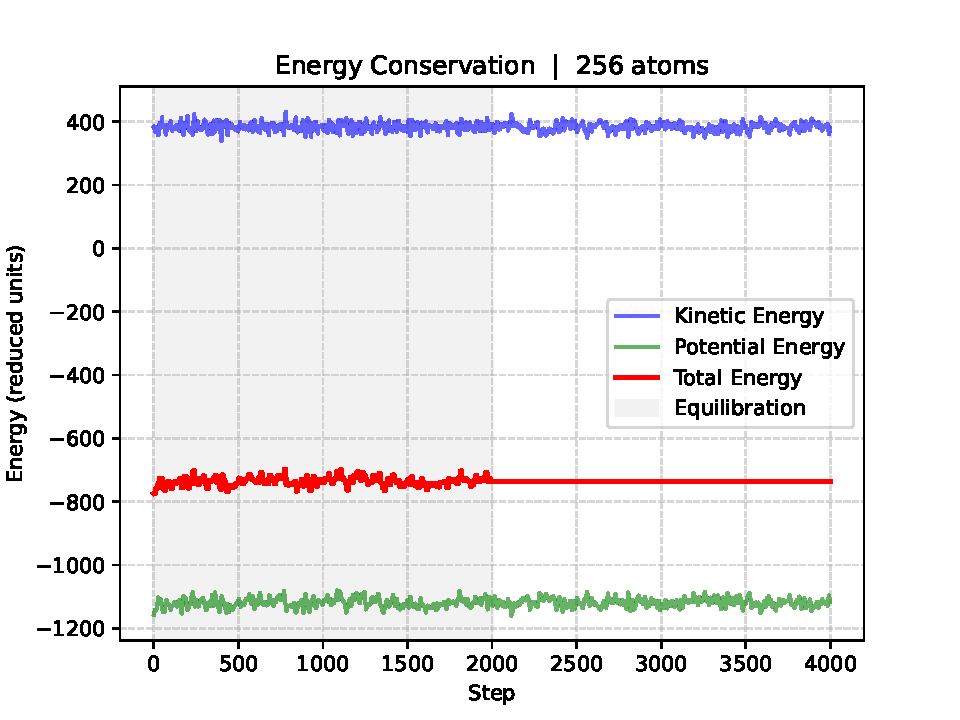
\includegraphics[width=\linewidth]{figures/energy_plot.pdf}
    \caption{Total energy $\Estar$, kinetic energy $K^*$, and potential
    energy $U^*$ as a function of timestep ($N = 256$, $\Tstar = 1.0$,
    $dt^* = 0.005$). During equilibration (steps 0--2000), velocity
    rescaling pins $K^*$ to the target; in the production phase
    (steps 2000--4000), all quantities evolve freely under NVE. The
    total energy $\Estar$ shows no systematic drift in the production
    phase, confirming integrator stability.}
    \label{fig:diag_energy}
\end{figure}

The diagnostic for energy conservation is evaluated exclusively during the production phase (steps 2000--4000). During equilibration, the active velocity rescaling thermostat continually alters the kinetic energy to drive the system to the target temperature, physically preventing energy conservation. Once rescaling is disabled for the production phase, the system evolves freely as an isolated microcanonical (NVE) ensemble. It is only in this unforced state that total energy must remain strictly constant, which is confirmed by the perfectly flat red line.

\subsection{Energy Fluctuation Metric}

In practice, floating-point arithmetic and the finite timestep introduce
small, bounded oscillations in $\Estar$. The simulation is considered
numerically stable when these fluctuations satisfy:
\begin{equation}
    \frac{\Delta \Estar}{\langle \Estar \rangle} \lesssim 10^{-4}
    \label{eq:fluct_criterion}
\end{equation}
where $\Delta \Estar = \sqrt{\langle (\Estar - \langle \Estar \rangle)^2 \rangle}$
is the root-mean-square fluctuation computed over the production phase only.
All quantities are reported both as totals and on a per-atom basis; the
per-atom values are more physically meaningful for comparison across
system sizes.

\begin{table}[H]
    \centering
    \caption{Energy stability metrics computed from the production phase
    (steps 2000--4000), $N = 500$, $\Tstar = 1.0$.}
    \label{tab:diag_energy}
    \begin{tabular}{lcc}
        \toprule
        \textbf{Quantity} & \textbf{Total} & \textbf{Per atom} \\
        \midrule
        Mean total energy $\langle \Estar \rangle$                      & $-734.935$  & $-1.4699$ \\
        RMS fluctuation $\Delta \Estar$                                 & $0.05138$   & $1.028 \times 10^{-4}$ \\
        Relative fluctuation $\Delta \Estar / |\langle \Estar \rangle|$ & \multicolumn{2}{c}{$6.99 \times 10^{-5}$} \\
        Criterion $\lesssim 10^{-4}$ satisfied?                         & \multicolumn{2}{c}{Yes} \\
        \bottomrule
    \end{tabular}
\end{table}

The relative fluctuation of $6.99 \times 10^{-5}$ comfortably satisfies
the $10^{-4}$ criterion, confirming that $dt^* = 0.005$ is a
sufficiently conservative timestep for this system.
\subsection{Zero Total Linear Momentum}

The total linear momentum of the system must remain zero throughout the
simulation as discussed in \ref{sec_Zero_net_momentum}.  Since every force on atom i from atom j is equal and opposite (Newton’s Third Law), $P^*$ should remain at machine precision\footnote{Machine precision is defined as the smallest representable positive number $\epsilon$ such that $1 + \epsilon \neq 1$ within the limits of the system's floating-point architecture.} for the
entire run once it is initialized to zero.

\begin{figure}[H]
    \centering
    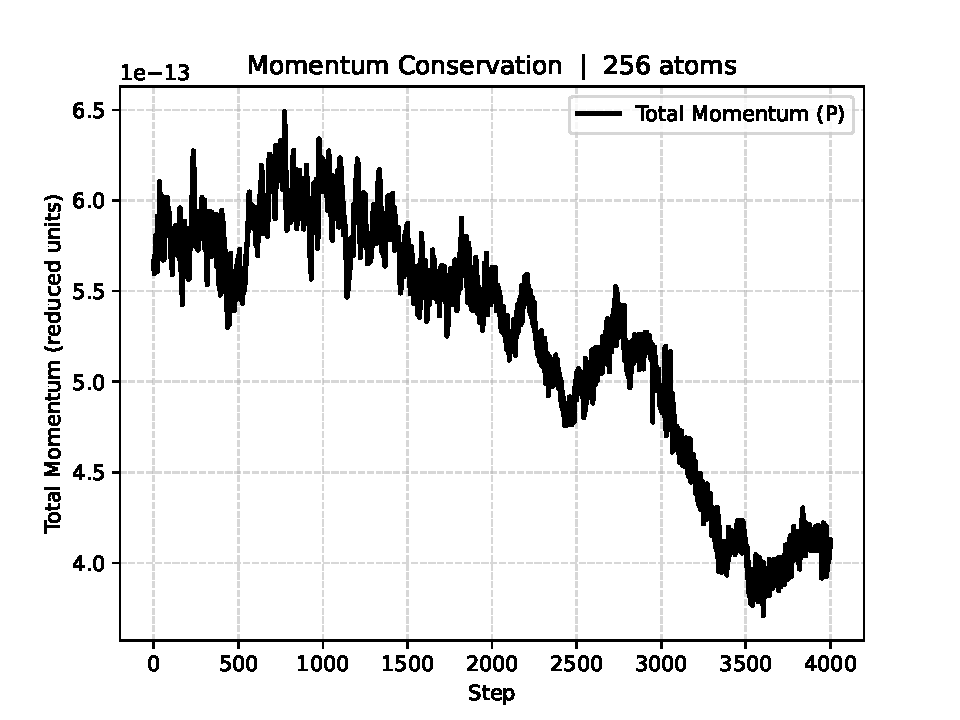
\includegraphics[width=0.8\linewidth]{figures/momentum_plot.pdf}
    \caption{Magnitude of total linear momentum $|\mathbf{P}^*|$ as a
    function of timestep ($N = 500$, $\Tstar = 1.0$). The value remains
    at $\sim 10^{-13}$ throughout, confirming that the velocity
    initialisation correctly eliminates net momentum and that the
    integrator preserves it.}
    \label{fig:diag_momentum}
\end{figure}

\begin{table}[H]
    \centering
    \caption{Maximum absolute value of each momentum component over the
    full simulation ($N = 256$, $\Tstar = 1.0$). All values are at
    floating-point machine precision ($\sim 10^{-13}$), confirming
    $\mathbf{P}^* \approx \mathbf{0}$.}
    \label{tab:diag_momentum}
    \begin{tabular}{lc}
        \toprule
        \textbf{Component} & \textbf{Max $|P^*|$ over full run} \\
        \midrule
        $P_x^*$ & $2.85 \times 10^{-13}$ \\
        $P_y^*$ & $2.17 \times 10^{-13}$ \\
        $P_z^*$ & $5.76 \times 10^{-13}$ \\
        \bottomrule
    \end{tabular}
\end{table}

All three momentum components stay around $10^{-13}$ throughout the simulation. The tiny fluctuations seen in Figure~\ref{fig:diag_momentum} are not physical; they are simply standard 64-bit floating-point rounding errors accumulating over the 4000 steps. Because these values are practically zero, the simulation cell remains effectively stationary.

\subsection{Summary}

All three stability criteria are satisfied. The total energy shows no
systematic drift in the production phase, with relative fluctuations of
$6.99 \times 10^{-5}$, well within the $10^{-4}$ threshold. The total
linear momentum remains at floating-point noise ($\sim 10^{-13}$)
throughout, confirming the centre-of-mass is stationary. The MD engine
is physically valid and numerically stable, and we proceed with extracting the
physical properties.